
\documentclass[11pt]{article}

\usepackage{common}
\title{HW4: Word Segmentation}
\author{Jeffrey Ling \\ jling@college.harvard.edu \and Rohil Prasad \\ prasad01@college.harvard.edu }
\begin{document}

\maketitle{}
\section{Introduction}

In this assignment, we examine the problem of word segmentation. Given a string of characters without spaces, we want to determine where we can insert spaces to segment the string into words. 

We implement and discuss several approaches to word segmentation in this paper, all trained on a portion of the Penn Treebank. Our first class of models are Markov models with emission distributions given by an n-gram count model and an adaptation of Bengio's neural network language model (NNLM). Our second class of models are recurrent neural networks (RNNs), namely the Long Short Term Memory (LSTM) network and the Gated Recurrent Unit (GRU) network. Furthermore, we attempt to optimize the evaluation algorithms used to construct segmentations given a model. For the Markovian models, we use a dynamic programming algorithm which greatly improves predictive accuracy. We also make a small adjustment to the RNN evaluation algorithm to improve the performance of these models as well. 

In Section 2, we give a formal description of our problem and establish our notation. In Section 3, we give detailed descriptions of the algorithms listed above. In Section 4, we present our experimental results. In Section 5, we discuss our findings.

\section{Problem Description}

Assume our training corpus consists of a sequence of characters $c_1, c_2, \dots, c_N$ where $c_i$ is drawn from a vocabulary $\mathcal{V}$ for every $i$. We use \texttt{<sp>} to denote the space character. 

Our training data represents this corpus as a pair of sequences $c_1, \ldots, c_N$ and $y_1, \ldots y_N$. The output variable $y_i \in \{0, 1\}$ indicates if character $c_{i+1}$ is a space. By default, we set $y_N = 1$ since $c_N$ is clearly not followed by a space. We desire to find a function $f : \mcV^k \to \mathbb{R}$ on sequences of characters that computes the probability of the next character being a space, i.e.
$$f(c_1, \ldots, c_k) = p(c_{k+1} = \texttt{<sp>} | c_1, \ldots, c_k) = p(y_k = 1 | c_1, \ldots, c_k)$$

In the test setup, calculating a word segmentation is equivalent to taking an input sequence of characters $\mathbf{c} \in \mcV^M$ without spaces and outputting a sequence $\mathbf{c}' \in \mcV^{M'}$ with spaces inserted, s.t. the corresponding sequence of indicators $\mathbf{y} = y_1y_2 \ldots y_{M'}$ has $y_i = 1$ iff $c_{i+1}'$ is a space.

We determine the \emph{best} word segmentation by finding the sequence $\mathbf{c}'$ with corresponding $\mathbf{y}$ that maximizes the score
$$\prod_{k=1}^{M'} p(y_k | c_1', \ldots, c_k') = \prod_{k=1}^{M'} f(c_1', \ldots, c_k') $$

For the approaches we are considering, this requires us to train a function $f$. Then, we apply an evaluation algorithm at test time (either based on greedy or dynamic programming) to generate such a segmented sequence. See Section 3 for details.

\subsection{Evaluation}

We evaluate our models on a validation set in two different ways. The validation set, a sequence of characters with spaces, can be considered as either a single sequence or a set of sentences.

First, we interpret our model as a language model that takes in a sequence of characters $c_1, \ldots, c_i$ and outputs a probability on the next character being a space, i.e. $p(c_{i+1} = \texttt{<sp>} | c_i \ldots c_1)$. Therefore, we can calculate perplexity over the validation set as a single sequence. This is equal to the exponential of the average negative log likelihood,
$$PPL = \exp\left(-\frac{1}{N} \sum_{i=1}^N \log p(c_{i+1} = \texttt{<sp>} | c_i \ldots c_1)\right)$$

Second, we can run our model and evaluation algorithm to get a word segmentation over the entire set. Here, we keep track of the number of spaces inserted into each sentence, then compute the mean squared error (MSE) with respect to the true number of spaces per sentence. This is the Kaggle metric.

\section{Model and Algorithms}

\subsection{Markovian Models}

The key to training tractable models is the Markov assumption. This allows us to get a simple expression for the joint probability that we can calculate using either a count-based model or a windowed feedforward neural network model. Recall that we desire to model
$$p(c_i = \texttt{<sp>} | c_1, \ldots, c_{i-1}) = p(y_i = 1 | c_1, \ldots, c_{i-1})$$

Under the Markov assumption, we only need to consider the last $n-1$ characters, so that we only need to model
\begin{equation}\label{eq:prob}
p(c_i = \texttt{<sp>} | c_{i-1}, \ldots, c_{i-n+1}) = p(y_i = 1 | c_{i-1}, \ldots, c_{i-n+1})
\end{equation}

We call models with such an assumption an n-gram model.

\subsubsection{Count Model}

To model equation~\ref{eq:prob} as an n-gram model, we compute co-occurrence counts $C(c_i = \texttt{<sp>}, c_{i-1}, \ldots, c_{i-n+1})$ and $C(c_i \neq \texttt{<sp>}, c_{i-1}, \ldots, c_{i-n+1})$ in the training sequence. Then with a smoothing parameter $\alpha$, we let
$$p(c_i = \texttt{<sp>} | c_{i-1}, \ldots, c_{i-n+1}) = \frac{\alpha + C(c_i = \texttt{<sp>}, c_{i-1}, \ldots, c_{i-n+1})}{2\alpha + C(c_i = \texttt{<sp>}, c_{i-1}, \ldots, c_{i-n+1}) + C(c_i \neq \texttt{<sp>}, c_{i-1}, \ldots, c_{i-n+1})}$$

For our models we set $\alpha = 0.1$.

\subsubsection{Neural Network Language Model (NNLM)}

We use Bengio's language model like last assignment to model equation~\ref{eq:prob}. We have parameters
\begin{itemize}
  \item $W_0 \in \mathbb{R}^{|\mathcal{V}| \times d_{in}}$, a lookup table of character embeddings
  \item $W_1 \in \mathbb{R}^{nd_{in} \times d_{hid}}$, $b_1 \in \mathbb{R}^{d_{hid}}$,
  \item $W_2 \in \mathbb{R}^{d_{hid} \times 2}$, $b_2 \in \mathbb{R}^{2}$
\end{itemize}

First, the character context is transformed into character embeddings by multiplying with $W_0$, and then concatenated to get a vector $\mathbf{x}_0$ of size $n \cdot d_{in}$. Then, we get a size $2$ vector of scores
$$\mathbf{z} = \text{tanh}(\mathbf{x}_0W_1 + b_1)W_2 + b_2 \in \mathbb{R}^2$$

Finally, we can force a probability distribution by taking the softmax $\hat{y} = \text{softmax}(\mathbf{z})$. Then, we have the probability that the next word is a space is $\hat{y}_2$.

As hyperparameters, we set $d_{in} = 15, d_{hid} = 100$, and we used a gram size of 5.

\subsection{Recurrent Neural Networks}

Our recurrent neural networks have the following parameters:
\begin{itemize}
  \item $W_0 \in \mathbb{R}^{|\mathcal{V}| \times d_{in}}$,
  \item $\mathbf{s}_0 \in \mathbb{R}^{d_{hid}}$, the initial hidden state,
  \item $R: \mathbb{R}^{d_{hid}} \times \mathbb{R}^{d_{in}} \to \mathbb{R}^{d_{hid}}$, a parameterized state transition function,
  \item $W_1: \mathbb{R}^{d_{hid}} \to \mathbb{R}^2$, $b_1 \in \mathbb{R}^{2}$
\end{itemize}

The exact definition of $R$ depends on the type of RNN we are using. All of our RNNS are \textbf{transducer} RNNs, meaning that they consume an input sequence $c_1, \dots, c_M$ of characters and output a sequence $\hat{y}_1, \dots, \hat{y}_M$, where $\hat{y}_i = p(y_i | c_i, c_{i-1}, \dots, c_1)$. 

\subsubsection{Long Short Term Memory Network}

We use the LSTM model of Hochreiter and Schmidhuber, illustrated below:

\begin{center}
  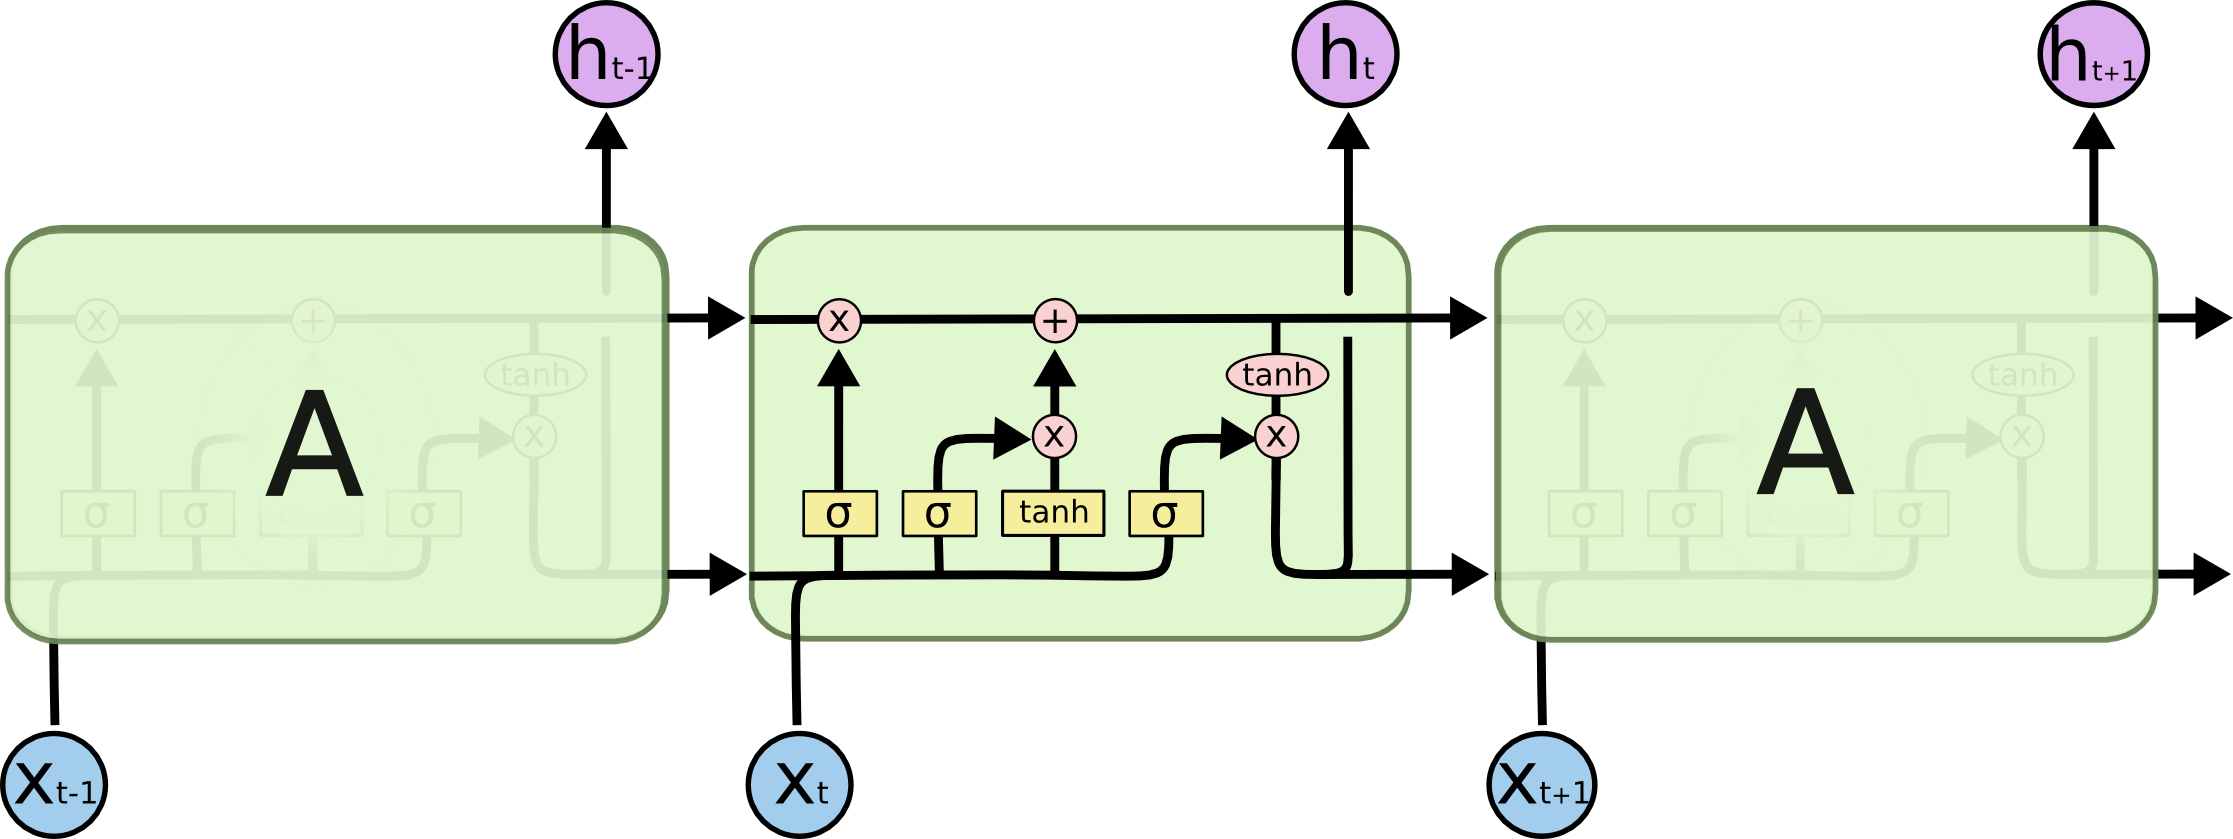
\includegraphics[width=0.5\textwidth]{LSTM3-chain.png}
\end{center}

Formally, this requires the introduction of some new parameters
\begin{itemize}
  \item $W^{xi} \in \mathbb{R}^{d_{in} \times d_{hid}}$, $W^{si} \in \mathbb{R}^{d_{hid} \times d_{hid}}$, $b^i \in \mathbb{R}^{d_{hid}}$, 
  \item $W^{xi} \in \mathbb{R}^{d_{in} \times d_{hid}}$, $W^{sj} \in \mathbb{R}^{d_{hid} \times d_{hid}}$, $b^j \in \mathbb{R}^{d_{hid}}$,
  \item $W^{xi} \in \mathbb{R}^{d_{in} \times d_{hid}}$, $W^{sf} \in \mathbb{R}^{d_{hid} \times d_{hid}}$, $b^f \in \mathbb{R}^{d_{hid}}$,
  \item $W^{xi} \in \mathbb{R}^{d_{in} \times d_{hid}}$, $W^{so} \in \mathbb{R}^{d_{hid} \times d_{hid}}$, $b^o \in \mathbb{R}^{d_{hid}}$,
  \item $\mathbf{C}_0 \in \mathbb{R}^{d_{hid}}$, the initial cell state
\end{itemize}

Let $c_i$ be our input character, and let $\mathbf{C}_{i-1}$ and $\mathbf{s}_{i-1}$ be the previously calculated cell and hidden states, respectively. First, we transform $c_i$ into a vector $\mathbf{x}_i$ of size $d_{in}$ by multiplying it by $W_0$. Then, we calculate the four following vectors
\begin{align*}
  \mathbf{i} &= \text{tanh}(\mathbf{x}_iW^{xi} + \mathbf{s}_{i-1}W^{si} + b^i) \\
  \mathbf{j} &= \sigma(\mathbf{x}_iW^{xj} + \mathbf{s}_{i-1}W^{sj} + b^j) \\
  \mathbf{f} &= \sigma(\mathbf{x}_iW^{xf} + \mathbf{s}_{i-1}W^{sf} + b^f) \\
  \mathbf{o} &= \sigma(\mathbf{x}_iW^{xo} + \mathbf{s}_{i-1}W^{so} + b^o) \\
\end{align*}
and combine them to produce the new cell state and hidden state
\begin{align*}
  \mathbf{C}_i &= \mathbf{j} \odot \mathbf{i} + \mathbf{f} \odot \mathbf{C}_{i-1} \\
  \mathbf{s}_i &= R(\mathbf{s}_{i-1}, \mathbf{x}_i) = \text{tanh}(\mathbf{C}_i) \odot \mathbf{o}
\end{align*}
Then, we multiply $\mathbf{s}_i$ by $W_1$ to produce an output vector $\mathbf{z}_i$ of size $2$. Finally, we force a probability distribution by taking the softmax to get the desired output $\hat{y}_i = \text{softmax}(\mathbf{z}_i)$. 

As hyperparameters, we use $d_{in} = 15, d_{hid} = 100$ as in the NNLM.

\subsubsection{Gated Recurrent Unit Network}

We use the GRU model of Cho et al. This model requires the following parameters in addition to the generic RNN parameters
\begin{itemize}
  \item $W^{xt} \in \mathbb{R}^{d_{in} \times d_{hid}}$, $W^{st} \in \mathbb{R}^{d_{hid} \times d_{hid}}$, $b^t \in \mathbb{R}^{d_{hid}}$, 
  \item $W^{xr} \in \mathbb{R}^{d_{in} \times d_{hid}}$, $W^{sr} \in \mathbb{R}^{d_{hid} \times d_{hid}}$, $b^r \in \mathbb{R}^{d_{hid}}$, 
  \item $W^x \in \mathbb{R}^{d_{in} \times d_{hid}}$, $W^s \in \mathbb{R}^{d_{hid} \times d_{hid}}$, $b \in \mathbb{R}^{d_{hid}}$
\end{itemize}

Let $c_i$ be our input character, and let $\mathbf{s}_{i-1}$ be the previously calculated hidden state. First, we transform $c_i$ into a vector $\mathbf{x}_i$ of size $d_{in}$ by multiplying it by $W_0$. Then, we calculate the following three vectors
\begin{align*}
  \widetilde{\mathbf{h}} &= \text{tanh}(\mathbf{x}_iW^{x} + (\mathbf{r} \odot \mathbf{s}_{i-1})W^s + b) \\
  \mathbf{r} &= \sigma(\mathbf{x}_iW^{xr} + \mathbf{s}_{i-1}W^{sr} + b^r) \\
  \mathbf{t} &= \sigma(\mathbf{x}_iW^{xt} + \mathbf{s}_{i-1}W^{st} + b^t)
\end{align*}
and combine them to produce the new hidden state
\begin{align*}
  \mathbf{s}_i &= R(\mathbf{s}_{i-1}, \mathbf{x}_i) = (1 - \mathbf{t}) \odot \widetilde{\mathbf{h}} + \mathbf{t} \odot \mathbf{s}_{i-1}
\end{align*}
Then, we multiply $\mathbf{s}_i$ by $W_1$ to produce an output vector $\mathbf{z}_i$ of size $2$. Finally, we force a probability distribution by taking the softmax to get the desired output $\hat{y}_i = \text{softmax}(\mathbf{z}_i)$. 
\subsection{Evaluation Algorithms}

We have three different algorithms that we use to take a model and use it to predict a sequence $y_1\dots y_M$ for an input sequence $c'_1\dots c'_M$. The first two are a greedy algorithm and a dynamic programming algorithm for our Markovian models. The last one is a greedy algorithm for our RNN models. In all of them, we will denote our model by a function $f$ from the input space to the space/non-space probability distribution. 

\subsubsection{Markovian Greedy}

%The algorithm is given formally. It simply consists of greedily predicting each $y_i$ and recording how many $y_i = 1$ per sentence. 
%
%\begin{algorithmic}
%  \Procedure{MarkovGreedy}{$(c_1, \dots, c_M)$, $f$}
%    \State{$sn \leftarrow 1$}
%    \Comment{Set sentence number to $1$}
%    \State{$S = \{\}$}
%    \Comment{Initialize empty dictionary}
%    \For{$i \in 1, \dots, M$}
%      \If{$c'_i = </s>$}
%        \State{$sn \leftarrow sn + 1$}
%        \State{$S[sn] \leftarrow 0$}
%        \Comment{Increment sentence number at end of sentence}
%      \EndIf{}
%      \State{$y \leftarrow f(c'_i)_2$}
%      \Comment{Feed $c'_i$ into the model}
%      \If{$y \geq 1/2$}
%        $S[sn] \leftarrow S[sn] + 1$
%      \EndIf{}
%    \EndFor{}
%    \Return{$S$}
%  \EndProcedure{}
%\end{algorithmic}

Given a sequence without spaces $c_1, \ldots, c_M$, we proceed greedily as follows. Given a context $c_{i-n+1}, \ldots, c_{i-1}$, we compute $p(c_i = \texttt{<sp>} | c_{i-1} \ldots c_{i-n+1})$. If this is greater than $0.5$, we insert a space and repeat with context $c'_{i-n+1}, \ldots, c'_{i-1}$ with $c'_{i-1} = \texttt{<sp>}$ and $c'_j = c_{j+1}$; otherwise we set $c'_{i-1}$ as the next character in the sequence.

In this manner we can process the entire test sequence to output spaces.

\subsubsection{Markovian Dynamic Programming}

Dynamic programming seeks to optimize the joint probability of a sequence with spaces:
$$\prod_{i=1}^{N} p(c_i = \texttt{<sp>} | c_{i-1}, \ldots, c_{i-n+1})$$
Note that for a bigram model, if we assume that spaces cannot follow spaces, this probability can be optimized by the greedy algorithm (since the only terms in this probability are of the form $p(c_i = \texttt{<sp>} | c_{i-1})$ for $c_{i-1}$ a non-space).

In a general n-gram model, we use a version of the Viterbi algorithm. We keep a table $\pi(i, B)$ where $B = y_{i-n+1} \ldots y_i$ is a bitmask of length $n$. The bits of $B$, $y_i$, indicate which characters in the original sequence $c_{i-n+1}, \ldots, c_{i-1}, c_i$ have a space following. Then $\pi(i, B)$ is equal to the joint log probability of the sequence $c_1, \ldots, c_i$ with final indicators of spaces $B = y_{i-n+1} \ldots y_i$.

The Viterbi transition is then given by the recursion
$$\pi(i, B) = \max_{B'} \pi(i-1, B') + g(\mathbf{c}_{(i-n+1):i}, B, B')$$
Here, $B'$ is a bitmask which has the last $n-1$ bits equalling the first $n-1$ bits of $B$, and $g(\mathbf{c}_{(i-n+1):i}, B, B')$ gives
$$\log p(y_i | c_i, \ldots, c_{i-n+1}, y_{i-1}, \ldots, y_{i-n+1})$$
Note that this probability only depends on the previous $n-1$ characters as determined by the $c_j$ and spaces $y_j$.

We can compute the optimal insertion of spaces by computing the table for $\pi$ and saving backpointers.

\subsubsection{RNN Greedy}

The algorithm is given formally below. In plain language, we simply feed in each character one at a time to our RNN. We set a cutoff probability $\mu \in (0, 1)$, so that we insert a space if the RNN outputs probability $> \mu$ of the next character being space. If the RNN predicts a space, we record that in our output dictionary, feed the space back into the RNN, and then continue to the next character. 

\begin{algorithmic}
  \Procedure{RNNGreedy}{$c'_1, \dots, c'_M$, $f$, $\mu$}
    \State{$i \leftarrow 1$}
    \State{$sn \leftarrow 1$}
    \Comment{Set sentence number to $1$}
    \State{$S = \{\}$}
    \Comment{$S$ maps sentences to number of spaces predicted}
    \State{$S[sn] = 0$}
    \While{$i \leq M$}
      \If{$c'_i = </s>$}
        \State{$sn \leftarrow sn + 1$}
        \State{$S[sn] \leftarrow 0$}
        \Comment{Increment sentence number at end of sentence}
      \EndIf{}
      \State{$y \leftarrow f(c'_i)_2$}
      \Comment{Feed $c'_i$ into the model}
      \If{$y \geq \mu$}
        \State{$y \leftarrow f(<sp>)$}
        \State{$S[sn] = S[sn] + 1$}
        \Comment{Feed a space into the model}
      \EndIf{}
      \State{$i \leftarrow i+1$}
    \EndWhile{}
  \Return{$S$}
  \EndProcedure{}
\end{algorithmic}

\section{Experiments}

We evaluate train and valid perplexity for all models. Table~\ref{tab:results} summarizes results.

\begin{table}[h]
\centering
\begin{tabular}{llcc}
 \toprule
 Model &  & Train PPL & Valid PPL \\
 \midrule
 \textsc{2-gram Count} & &1.397 & 1.400 \\
 \textsc{3-gram Count} & &1.267 & 1.273 \\
 \textsc{4-gram Count} & &1.173 & 1.183  \\
 \textsc{5-gram Count} & &1.122 & 1.149 \\
 \textsc{6-gram Count} & &1.102 & 1.168 \\
 \textsc{NNLM} & & 1.153 & 1.162 \\
 \textsc{LSTM} & & 1.110 & 1.142 \\
 \textsc{GRU} &  & 1.097 & 1.138 \\
 \bottomrule
\end{tabular}
\caption{\label{tab:results} Perplexity on space insertion.}
\end{table}

After training, we also record the MSE for each model on valid with both greedy and dynamic programming test methods. Table~\ref{tab:mse} summarizes results.

\begin{table}[h]
\centering
  \begin{tabular}{ ccc}
    \hline Model &  & MSE \\
    \hline 5-gram Count+Greedy & & 23.67\\
    5-gram Count+DP & & 3.20 \\
    NNLM+Greedy & & 15.14\\
    NNLM+DP & & 11.26 \\
    LSTM &  & 5.42 \\
    GRU &  & 5.26 \\
    \hline
  \end{tabular}
\caption{MSE on space insertion for valid. The RNNs used $\mu = 0.3$ as cutoff probability.}
\label{tab:mse} 
\end{table}

\subsection{Count Model}

For the count model, we experiment with the gram size up to 5. We use smoothing $\alpha = 0.1$. We find that 5-gram gets the best valid perplexity, so we use this for the NNLM as well.

\subsection{NNLM}

For the NNLM, we trained with hidden size 100, word embedding size 15, learning rate 0.01, batch size 32, and trained for 10 epochs (upon which validation perplexity stopped decreasing). We used a context size (i.e. gram size) of 5. The NNLM takes about 30 seconds to train per epoch.

\subsection{RNN}

For both the LSTM and GRU, we trained with hidden size 100, word embedding size 15, learning rate 0.1, batch size 32, and trained for 20 epochs. We track validation perplexity per epoch and halve learning rate if it stops decreasing (though this wasn't necessary in 20 epochs). The LSTM and GRU both take about 30 seconds per training epoch.


\begin{figure}[h]
\centering
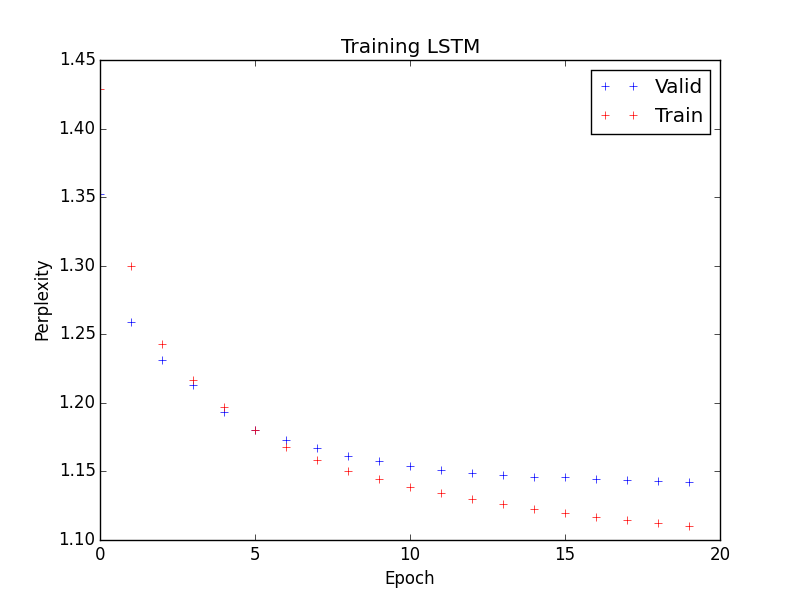
\includegraphics[scale=0.5]{train_lstm}
\caption{Training curves for LSTM.}
\end{figure}

\begin{figure}[H]
\centering
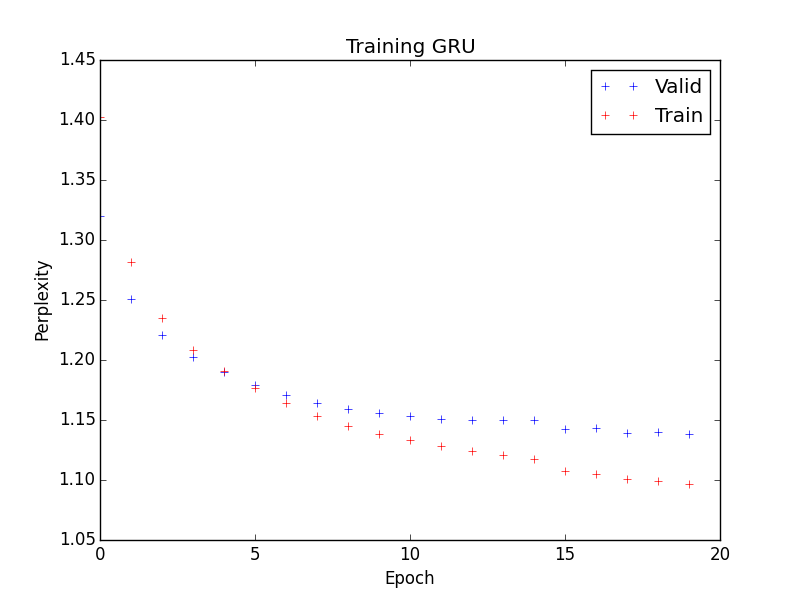
\includegraphics[scale=0.5]{train_gru}
\caption{Training curves for GRU.}
\end{figure}

We experimented with the cutoff probability $\mu$ for the LSTM. We find that MSE on valid is optimized at $\mu = 0.3$, which was optimized by grid search on the LSTM trained for $20$ epochs. The results are given in the figure below.  %% plot this?

\begin{figure}[H]
\centering
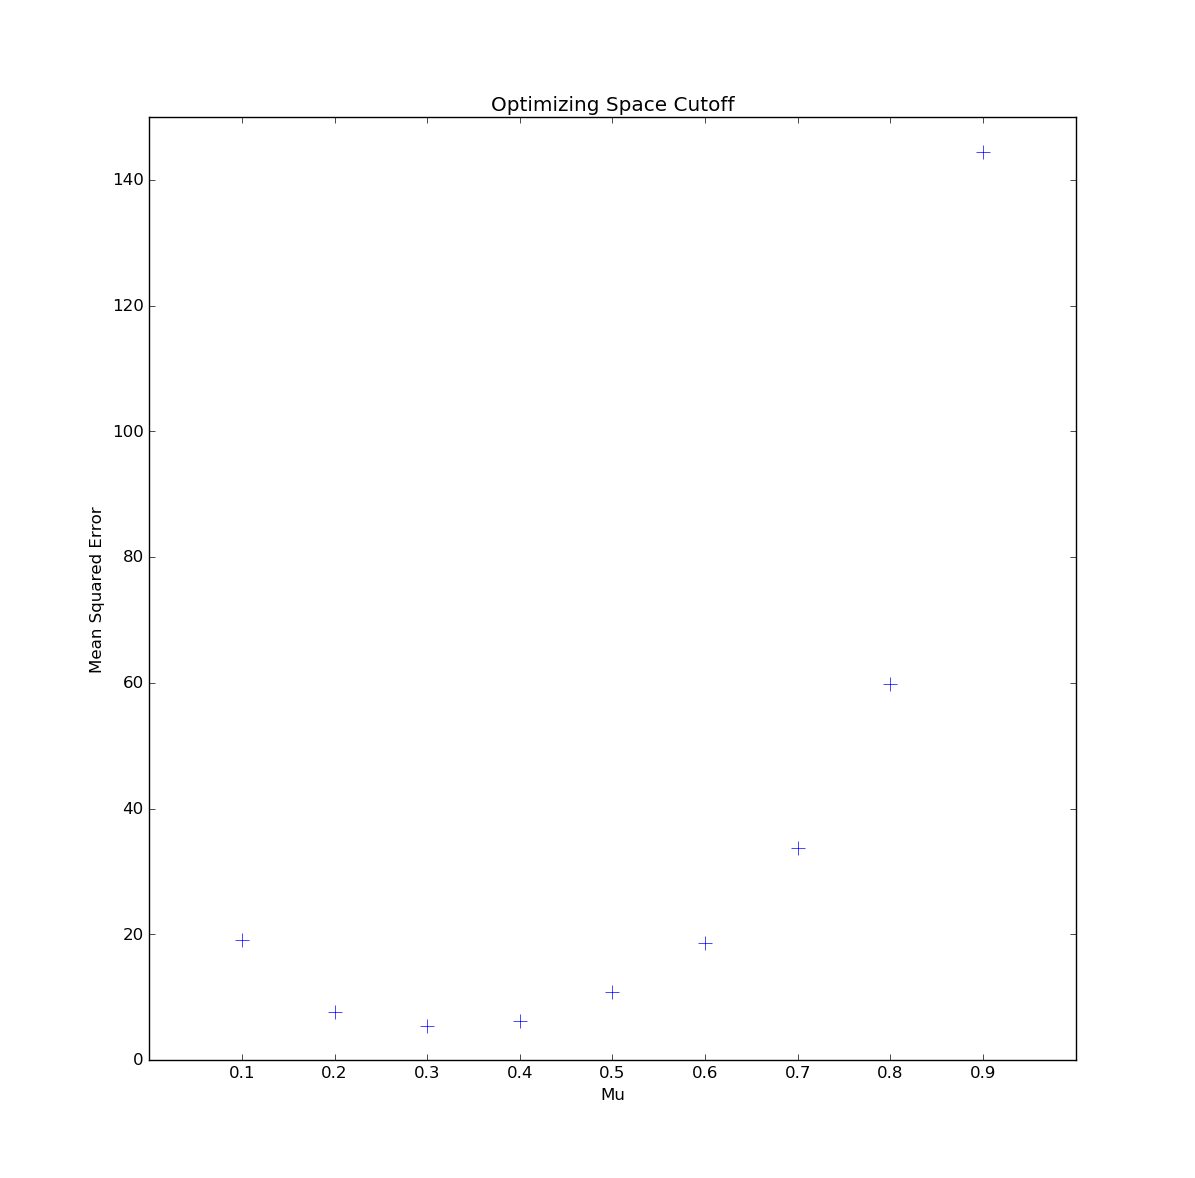
\includegraphics[scale=0.4]{mu_plot}
\caption{Grid search for $\mu$}
\end{figure}

%\begin{center}
%\begin{tabular}{ c c}
%  \hline $\mu$ & MSE \\
%  \hline $0.1$ & 19.1\\
%  $0.2$ & 7.7\\
%  $0.3$ & 5.4\\
%  $0.4$ & 6.3\\
%  $0.5$ & 10.9\\
%  $0.6$ & 18.6\\
%  $0.7$ & 33.6\\
%  $0.8$ & 59.8\\
%  $0.9$ & 144.4\\
%  \hline
%\end{tabular}
%\end{center}

\section{Conclusion}



\bibliographystyle{apalike}
\bibliography{writeup}

\end{document}
